\documentclass[journal]{journal}
\usepackage{subcaption}
\usepackage{graphicx}
\usepackage{url}
\usepackage{color}
\usepackage{multirow}
\usepackage{makecell}
\usepackage{mathptmx}
\usepackage{amsmath}
%define some own functions
\newcommand{\tabincell}[2]{\begin{tabular}{@{}#1@{}}#2\end{tabular}} 
\def\D{\mathrm{d}}
% correct bad hyphenation here
\hyphenation{op-tical net-works semi-conduc-tor}
\pagestyle{empty}
\begin{document}

\title{Invariant Object Recognition using Spiking Neurons}
\author{
Qian~Liu
%and~Steve~Furber,~\IEEEmembership{Fellow,~IEEE}
%\thanks{
%The authors are with the School of Computer Science, University of Manchester, Manchester M13 9PL, U.K. 
%(e-mail:qian.liu-3@manchester.ac.uk; steve.furber@manchester.ac.uk).}
}% <-this % stops a space
%\thanks{Manuscript received April 19, 2005; revised January 11, 2007.}}

\maketitle
\thispagestyle{empty}

\begin{abstract}
%The human brain recognises huge amount of objects rapidly with ease even in cluttered and natural scenes.
%This robust object recognition of the biological system is invariant to the change of position, scale, viewing angle and etc. 
%(known as transformation invariance).
%While 
The major stumbling problem of the computer object recognition lies in the poor robustness to the transformations.
Exploring and mimicking invariant object recognition within the brain is a promising approach to tackling the computational difficulty;
in turn it also contributes to the understanding biological visual processing by means of mimicking neural activity in the brain.

Thanks to its high-performance massively parallel processing, SpiNNaker makes it possible to simulate large-scale neural networks in real-time.
%Thus, in order to explore the ventral visual pathway of primate brain, this work hires a neuromorphic hardware system formed from a Dynamic Video Sensor~(DVS) silicon retina in concert with SpiNNaker.
As a first milestone of this study, a recognition system for dynamic hand postures is developed on a neuromorphic hardware platform. Future work is proposed to build an object recognition system with position, scale and view invariance by modelling the hierarchical visual pathway up to the inferotemporal (IT) cortex.
The proposed plan of the system will be able to recognise 200 objects in real time exploiting Integrate-and-Fire(LIF) neurons.
\end{abstract}

%\begin{IEEEkeywords}
%spiking neural network (SNN), convolutional neural network (CNN), posture recognition, neuromorphic system.
%\end{IEEEkeywords}


\section{Introduction}
Patterns or objects in two-dimensional images can be described with four properties~\cite{wysoski2008fast}: position, geometry (i.e. size, area and shape), colour/texture, and trajectory. 
Appearance-based methods are the most direct approach to performing pattern recognition where the test image is compared with a set of templates to find the best match for an individual or combination of properties. 
%In terms of classification algorithms, distance measure methods (nearest neighbour, k-means clustering), support vector machine (SVM), multi-layer perceptron (MLP) neural networks and statistical methods, e.g. Gaussian mixture model (GMM) have been applied successfully in visual recognition. 
However, the 2D projection of an object changes under different conditions including illumination, viewing angles, relative positions and distance, making it virtually impossible to represent all appearances of an object. 
To improve reliability, robustness and classification efficiency, approaches such as edge matching~\cite{canny1986computational}, divide-and-conquer~\cite{toygar2004multiple}, gradient matching~\cite{wei2006robust} and feature based methods~\cite{lowe2004distinctive, bay2008speeded} are used.
%Moreover, feature based methods are used to improve reliability, robustness and classification efficiency. 
%Among various feature extraction methods, the scale-invariant feature transform (SIFT)~\cite{lowe2004distinctive} and the sped-up robust features (SURF)~\cite{bay2008speeded} methods are well-accepted recently in the field. 
Finding an appropriate feature for a specific object still remains an open question and there is no process as general, accurate, or energy-efficient as that demonstrated by the brain.
It is not a new idea to turn to nature for inspiration. 
%Turning to biology for answers is always the way to explore the field of visual pattern recognition. 
Riesenhuber et al.~\cite{riesenhuber1999hierarchical}, for instance, presented a biologically-inspired model based on the organisation of the visual cortex which has the ability to represent relative position- and scale-invariant features.
Integrating a rich set of visual features became possible using a feed-forward hierarchical pathway. 

\subsection{What Is Object Recognition?}
\label{sec:aim}
Object recognition is the process of assigning labels to particular objects, ranging from precise labels (`identification') to coarse labels (`categorisation')~\cite{dicarlo2012does}.
This includes the ability to accomplish these tasks under various identity preserving transformations such as object position, scale, viewing angle, background clutter and etc.

The brain can accurately recognise and categorise objects remarkably quickly, for example object recognition time in monkeys is under 200~ms~\cite{fabre1998rapid} and the images are presented sequentially in spikes less than 100~ms~\cite{keysers2001speed}.
This research focuses on this rapid and highly accurate object recognition, `core recognition', which is defined in~\cite{dicarlo2007untangling}.


\subsection{Why Is It Important?}
\label{sec:imp}
The human brain recognises huge amount of objects rapidly with ease even in cluttered and natural scenes.
This robust object recognition of the biological system is invariant to the change of position, scale, viewing angle and etc. (known as transformation invariance).
While the major stumbling problem of the computer object recognition lies in the poor robustness to the transformations.
Each encounter of an object on the retina is unique because of differing illumination (lighting conditions), position (projection locations on the retina), scale (distances and sizes), pose (viewing angles), and clutter (visual contexts).
In addition, a difficult specificity-invariance trade-off occurs in the categorisation tasks, since the recognition should be able to discriminate different object classes (intraclass variability) while at the same time remaining tolerant to image transformations.   

Exploring and mimicking invariant object recognition within the brain is a promising approach to tackling the computational difficulty;
in turn it also contributes to the understanding biological visual processing by means of mimicking neural activity in the visual system of the brain.
Moreover, energy-efficiency improvements following from the great energy efficiency of biological systems will help in building object recognition systems, e.g. posture recognition for human-machine interfaces in mobile devices.  

\subsection{How to Mimic The Brain?}
\label{sec:brn}
To explore how brain may recognise objects, we have employed a biologically-inspired DVS silicon retina~\cite{lenero20113}.
This is a good example of low-cost visual processing due to its event-driven and redundancy-reducing style of computation;
and a SpiNNaker system~\cite{furber2014spinnaker}, which is a massive parallel computing platform aimed at real-time simulation of SNNs. 
%SpiNNaker, as the back-end of the system, provides a flexible, event-driven mechanism for real-time simulation of SNNs, and is where the posture recogniser locates.
%Thanks to its high-performance massively parallel processing, SpiNNaker makes it possible to simulate large-scale neural networks in real-time.
Thanks to its high-performance processing of large-scale neural networks, we explore biological approaches of visual processing by mimicking the functions of different layers along the ventral visual pathway. 

Building a real-time recognition system for dynamic hand postures is a first step of exploring visual processing in a biological fashion and is also a validation of the performance of the neuromorphic platform.
%To match the image properties detailed earlier, the position, shape, size and trajectory of the hand postures can be detected from the retina output.
To keep the task simple at first, the postures are of similar size and the goal is to recognise the shape of a hand with moving positions.
This preliminary work achieved the first milestone of the research which aims at building a position-invariant object recognition system exploiting V1-like neurons (primary visual cortex: area V1) to classify five hand postures. 

\section{Biological Aspects}
\label{sec:bio}
The central visual system consists of several cortical areas responsible for visual processing, which are placed in a hierarchical pattern according to the anatomical experiments~\cite{felleman1991distributed}.
There are two basic streams locating in the visual area: a dorsal and a ventral pathway .% (Figure~\ref{Fig:TwoPath}).
This research mainly focuses on the ventral visual pathway, since it dominates the object recognition among the cortical areas.
%\begin{figure}[h!]
%	\centering
%	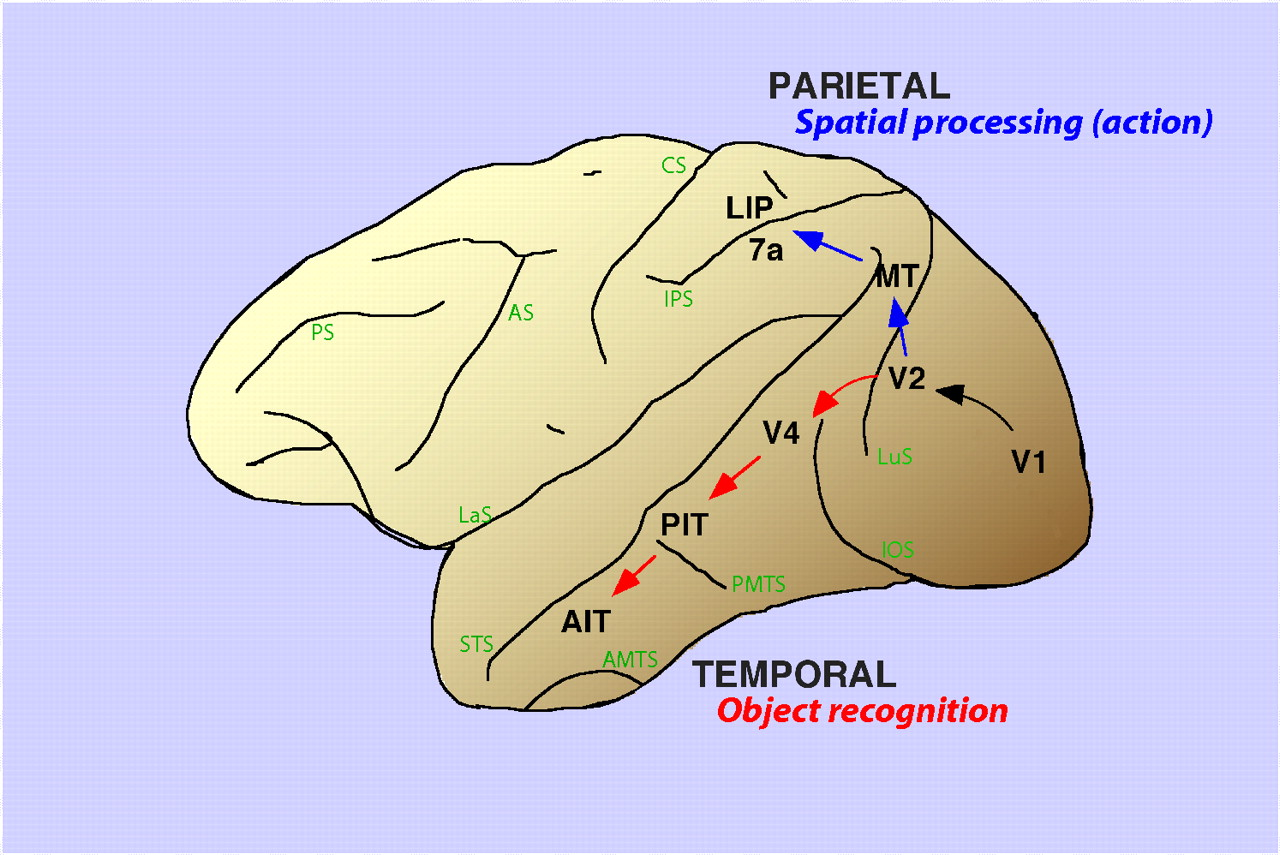
\includegraphics[width=0.48\textwidth]{pics/twoPaths.jpg}
%	\caption{The dorsal and ventral pathway in the brain~\cite{lehky2007comparison}.
%	The dorsal stream (blue) arrives to the parietal lobe, whereas the ventral pathway (red) reaches the inferotemporal (IT) cortex in the temporal lobe.}
%	\label{Fig:TwoPath}
%\end{figure}
\begin{figure}[h!]
	\centering
	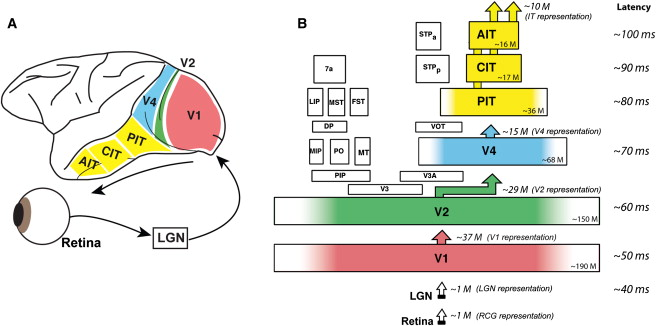
\includegraphics[width=0.48\textwidth]{pics/ventral.jpg}
	\caption{The ventral visual pathway and abstraction layers~\cite{dicarlo2012does}.
}
	\label{Fig:Ventral}
\end{figure}

\subsection{The ventral visual pathway}
The ventral visual pathway (Figure~\ref{Fig:Ventral}) starts from the primary visual cortex V1 in the occipital cortex through areas such as V2 and V4 to the Inferotemporal (IT) cortex.

\textbf{Primary Visual Cortex: V1.}
As the simplest and earliest cortical area in the ventral stream, the primary visual cortex V1 is the best-studied since the well-known discovery of the orientation selectivity by Hubel and Wiesel~\cite{hubel1959receptive} in 1958.
In the spatial domain, V1 neurons are tuned to Gabor-like transforms applied to their small local receptive field.
In theory, these Gabor-like filters together can carry out neuronal processing of spatial frequency, orientation, motion, direction, speed, and many other spatio-temporal features.

\textbf{Visual Areas V2/V4.}
%Visual area V2, also called prestriate cortex~\cite{an2012distinct}, is the second major area located in the occipital lobe of the primate brain, and the first region within the visual association area~\cite{wu2011early}. 
%It receives strong feed-forward connections from V1 and has many properties in common with V1. 
%The responses of V2 neurons are tuned to simple shapes such as orientation and sinusoidal gratings. 
%Moreover, V2 neurons are able to represent variety of higher order shapes that are based on contours (e.g., angles and curves with multiple orientations at different subregions within a single receptive field) or grating patterns~\cite{hegde2000selectivity}.
The responses of many V2 neurons are also modulated for complex properties: orientation of illusory contours~\cite{anzai2007neurons}, binocular disparity~\cite{daniel2009whither}, and whether the stimulus is part of the figure or the ground~\cite{qiu2005figure}.

%In a recent study, the Layer 6 cells of the V2 cortex were found to play a very important role in the storage of Object Recognition Memory as well as the conversion of short-term object memories into long-term memories.[23]
%
%\textbf{Visual Area V4.}
%Area V4 is the third cortical area in the ventral stream, receiving strong feedforward input from V2 and transmitting to the PIT.
%It also receives direct inputs from V1 which are mostly generated in the visual central space.
%V4 is the first area in the ventral stream to show strong attentional modulation.
%Most studies indicate that selective attention can change firing rates in V4 by about 20\%~\cite{filipe2013human}.
%This discovery found by Moran and Desimone~\cite{moran1985selective} was the first report of attention effects anywhere in the visual cortex.

Although V4 is mainly modulated for colour recognition, it is also tuned for orientation and spatial frequency similar to V1.
Comparing to V1, V4 responds to more complex object features with intermediate complexity.
% but is not tuned for complex objects as areas in the inferotemporal cortex are~\cite{williams2007biological}.

\textbf{Inferotemporal Cortex: IT.}
%Inferotemporal Cortex is only found in the temporal lobe in primates including humans. 
%It is tuned to a range of object features complexity starting with simpler patterns in the PIT/TEO~\cite{tanaka1991coding};
%And the 
The complexity increases along the ventral stream towards anterior IT (AIT) where objects are represented and recognised~\cite{dean1976effects}.
The high-order complex features includes the combinations of colour or texture with complicated shapes~\cite{tanaka1991coding}, and body parts such as faces and hands~\cite{gross2008single}.
The distinguishing features of the IT cortex is that the neuronal responses are position and size invariant~\cite{schwartz1983shape}, and also invariant to changes in luminance, texture, and relative motion ~\cite{sary1993cue}.
%It is wide-accepted that the identity-preserving transformation invariance makes IT ideal for representing objects despite changes in the surrounding environment and retinal image.

\subsection{Object Representation in IT}
The neuronal representation in the cortical area of IT is considered to be the spatio-temporal pattern of spikes.
The spiking activities of single neurons and populations are thought to hold the key to encode visual information.
\begin{figure}
	\centering
	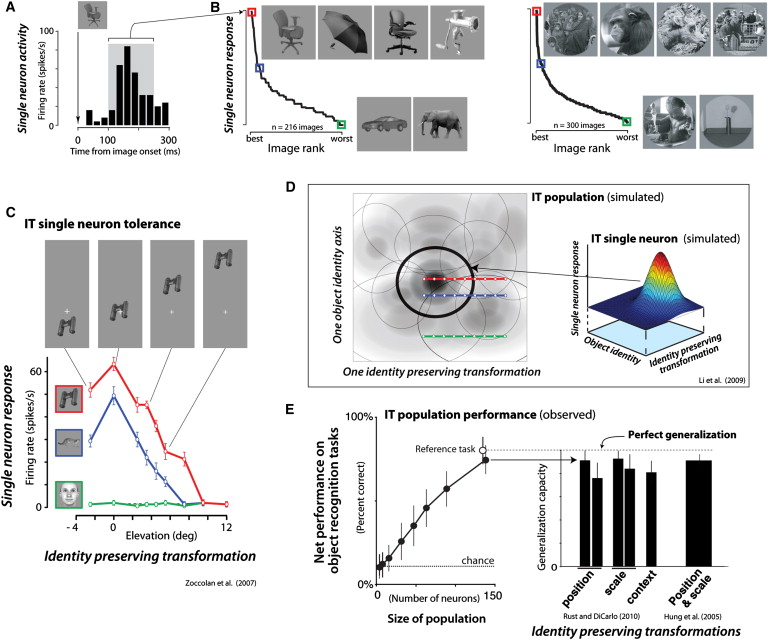
\includegraphics[width=0.48\textwidth]{pics/IT.jpg}
	\caption{	
		IT single-neuron properties and their relationship to population performance~\cite{dicarlo2012does}.
	}
	\label{Fig:IT}
\end{figure}


\textbf{Single neurons.}
Most studies have investigated the neural activities in the IT by means of firing rate or spike count.
A typical histogram, Figure~\ref{Fig:IT}(A)~\cite{zoccolan2007trade}, shows the spike count of a single neuron in time bins of 25~ms for a duration of 300~ms in total right after the presentation of a visual image.
The highlighted time window, the so-called `decoding' window, is adjusted to the latency of the conductance along the ventral stream. 
The spike count of the `decoding' window is well modulated for object identity, position or size~\cite{desimone1984stimulus}, see example in Figure~\ref{Fig:IT}(B) where the left shows the spiking activities for clean figures and the right for natural scenes.
The neural responses were sorted from high to low with the corresponding figures presented, where the red point indicated the highest respond while the green the lowest and the blue the medium.
Another example in Figure~\ref{Fig:IT}(C) shows the responses of an example IT neuron obtained by varying the position (elevation) of three objects with high (red), medium (blue), and low (green) activities.
The object identity preference was maintained in the entire test range regardless of the position changes.
%These tuning curves are similar to the well-understood firing rate modulation in visual area V1 on the bar orientation.

%Understanding IT single neuron responses has proven to be extremely challenging and even predicting the responses of an IT neuron to a new image remains impossible.
%Nevertheless, IT neurons are activated by complex combinations of visual features and that they are often able to maintain their relative object preference over small to moderate changes in object position, scale, pose~\cite{logothetis1996visual}, illumination~\cite{vogels2002effects} and clutter~\cite{zoccolan2005multiple}.

%respond to more objects\\
Although IT neurons are commonly described as narrowly selective object identifier, neurophysiological studies have shown a diverse selectivity of single neurons~\cite{desimone1984stimulus}.
%Most IT neurons are broadly tuned and the typical IT neuron responds to many different images and objects~\cite{zoccolan2007trade}, also see Figure~\ref{Fig:IT}(B).
As illustrated in Figure~\ref{Fig:IT}(D), a single neuron (right) is modulated to both object identities and variables of identity-preserving transformations.
%To explain the plot in ~\ref{Fig:IT}(C), position is the variable here; thus the tuning curve for different identities on each position can be described as a slice in the 3-D plot which is Gaussian-like.
%As a result, the rank order of the three objects remains the same due to the Gaussian-like curve stays similar.
%If a population of such IT neurons tiles with the overlapping fashion, see left panel of Figure~\ref{Fig:IT}(D), a more accurate recognition result containing the transformation parameter can be carried out with population coding.

\textbf{Population of neurons.}
%Spike timing variability in the ms resolution of spikes is consistent with a Poisson-like stochastic spike generation process.
%The underlying output rate of IT neurons is determined by each particular image.
%Despite the timing variability, the brain can reliably recognise the presented object by integrating the neural responses across IT population~\cite{de2007properties}.
%However, it still remains unclear whether the spike timing variability brings down the encoding/decoding accuracy or if it contributes to the population tuning for useful informations~\cite{ermentrout2008reliability}. 
Although the first stage of the ventral stream, V1, is reasonably well studied, the visual processing in higher stages especially in V4 and IT remains poorly understood.
Nevertheless, as stated above IT is the main part of ventral stream to recognise and categorise the objects in real-time and is tolerant to identity-preserving transformations.
Specifically, simple linear classifier built on the output rates of randomly selected population with only a few hundred neurons reveals a high-level of object recognition performance~\cite{hung2005fast};
and the simple weighted summation explains a wide range of invariant object recognition behaviour sufficiently~\cite{majaj2012unified}.

Figure~\ref{Fig:IT}(E) shows the direct tests of measuring the cross-validated population performance on categorisation tasks using linear classifiers.
The recognition performance approaches ceiling level with only a few hundred neurons (left panel), and the same population shows a good generalization across moderate changes in position, scale, and context.
%50 ms window matters\\

\textbf{Decoding Window Matters.}
The output spiking pattern of the ventral visual stream are well described by a firing rate code where the decoding window size is 50~ms~\cite{hung2005fast}.
Thus the visual representation in IT is usually found in the first 50~ms of neuronal response, although different time epochs relative to stimulus onset may encode different types of visual information~\cite{brincat2006dynamic} (see Figure~\ref{Fig:IT}(A), an appropriate decoding window can be 100-150~ms after image onset).

\subsection{Hierarchical Feed-forward Organisation }
In sum, the output of the ventral stream is reflexively expressed in neuronal firing rates across a short interval of 50 ms and is an explicit object representation;
and the rapid production of this representation is consistent with a largely feed-forward, non-linear processing of the visual input~\cite{dicarlo2012does}.

The corresponding hierarchical organisation is showed in Figure~\ref{Fig:Ventral}(B).
Each area is plotted with the size proportional to its cortical surface size.
Approximate total number of neurons of both hemispheres is shown in the corner of the cortical areas.
The approximate number of projections is written above each block.
In addition, the colour dedicates to processing the central 10$^\circ$ of the visual field.
At last, approximate median response latency is listed on the right.

\section{Preliminary Work}
To explore how the brain may recognise objects in its general,accurate and energy-efficient manner, this work employs a neuromorphic hardware system formed from a Dynamic Video Sensor~(DVS) silicon retina in concert with the SpiNNaker real-time Spiking Neural Network~(SNN) simulator.
Inspired by the behaviours of the primary visual cortex, Convolutional Neural Networks (CNNs) are modelled using both linear perceptrons and LIF neurons.

\subsection{Platform}
The outline of the platform is illustrated in Figure~\ref{fig:SysOverViewa}, where the hardware system is configured, controlled and monitored by the PC.
%Figure~\ref{fig:SysOverViewb} shows the combined hand posture recognition system; 
The jAER~\cite{delbruck2008frame} event-based processing software on the PC configures the retina and displays the output spikes through a USB link.
The host communicates to the SpiNNaker board via Ethernet to set up its runtime parameters and to download the neural network model off-line.
It visualises~\cite{6252490} the spiking activity of the network in real-time.
The photograph of the hardware platform, Figure~\ref{fig:SysOverViewb}, shows that the silicon retina connects to the SpiNNaker 48-node system via a Spartan-6 FPGA board~\cite{galluppi2012real}.
%, which was also applied to a sound localisation system.


\begin{figure}[h!]
\centering
	\begin{subfigure}[t]{0.48\textwidth}
		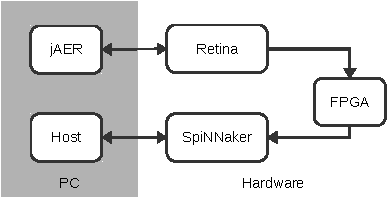
\includegraphics[width=\textwidth]{pics/outline.pdf}
	    \caption{Outline of the platform.}
	    \label{fig:SysOverViewa}
	\end{subfigure}
	\\
	\begin{subfigure}[t]{0.48\textwidth}
		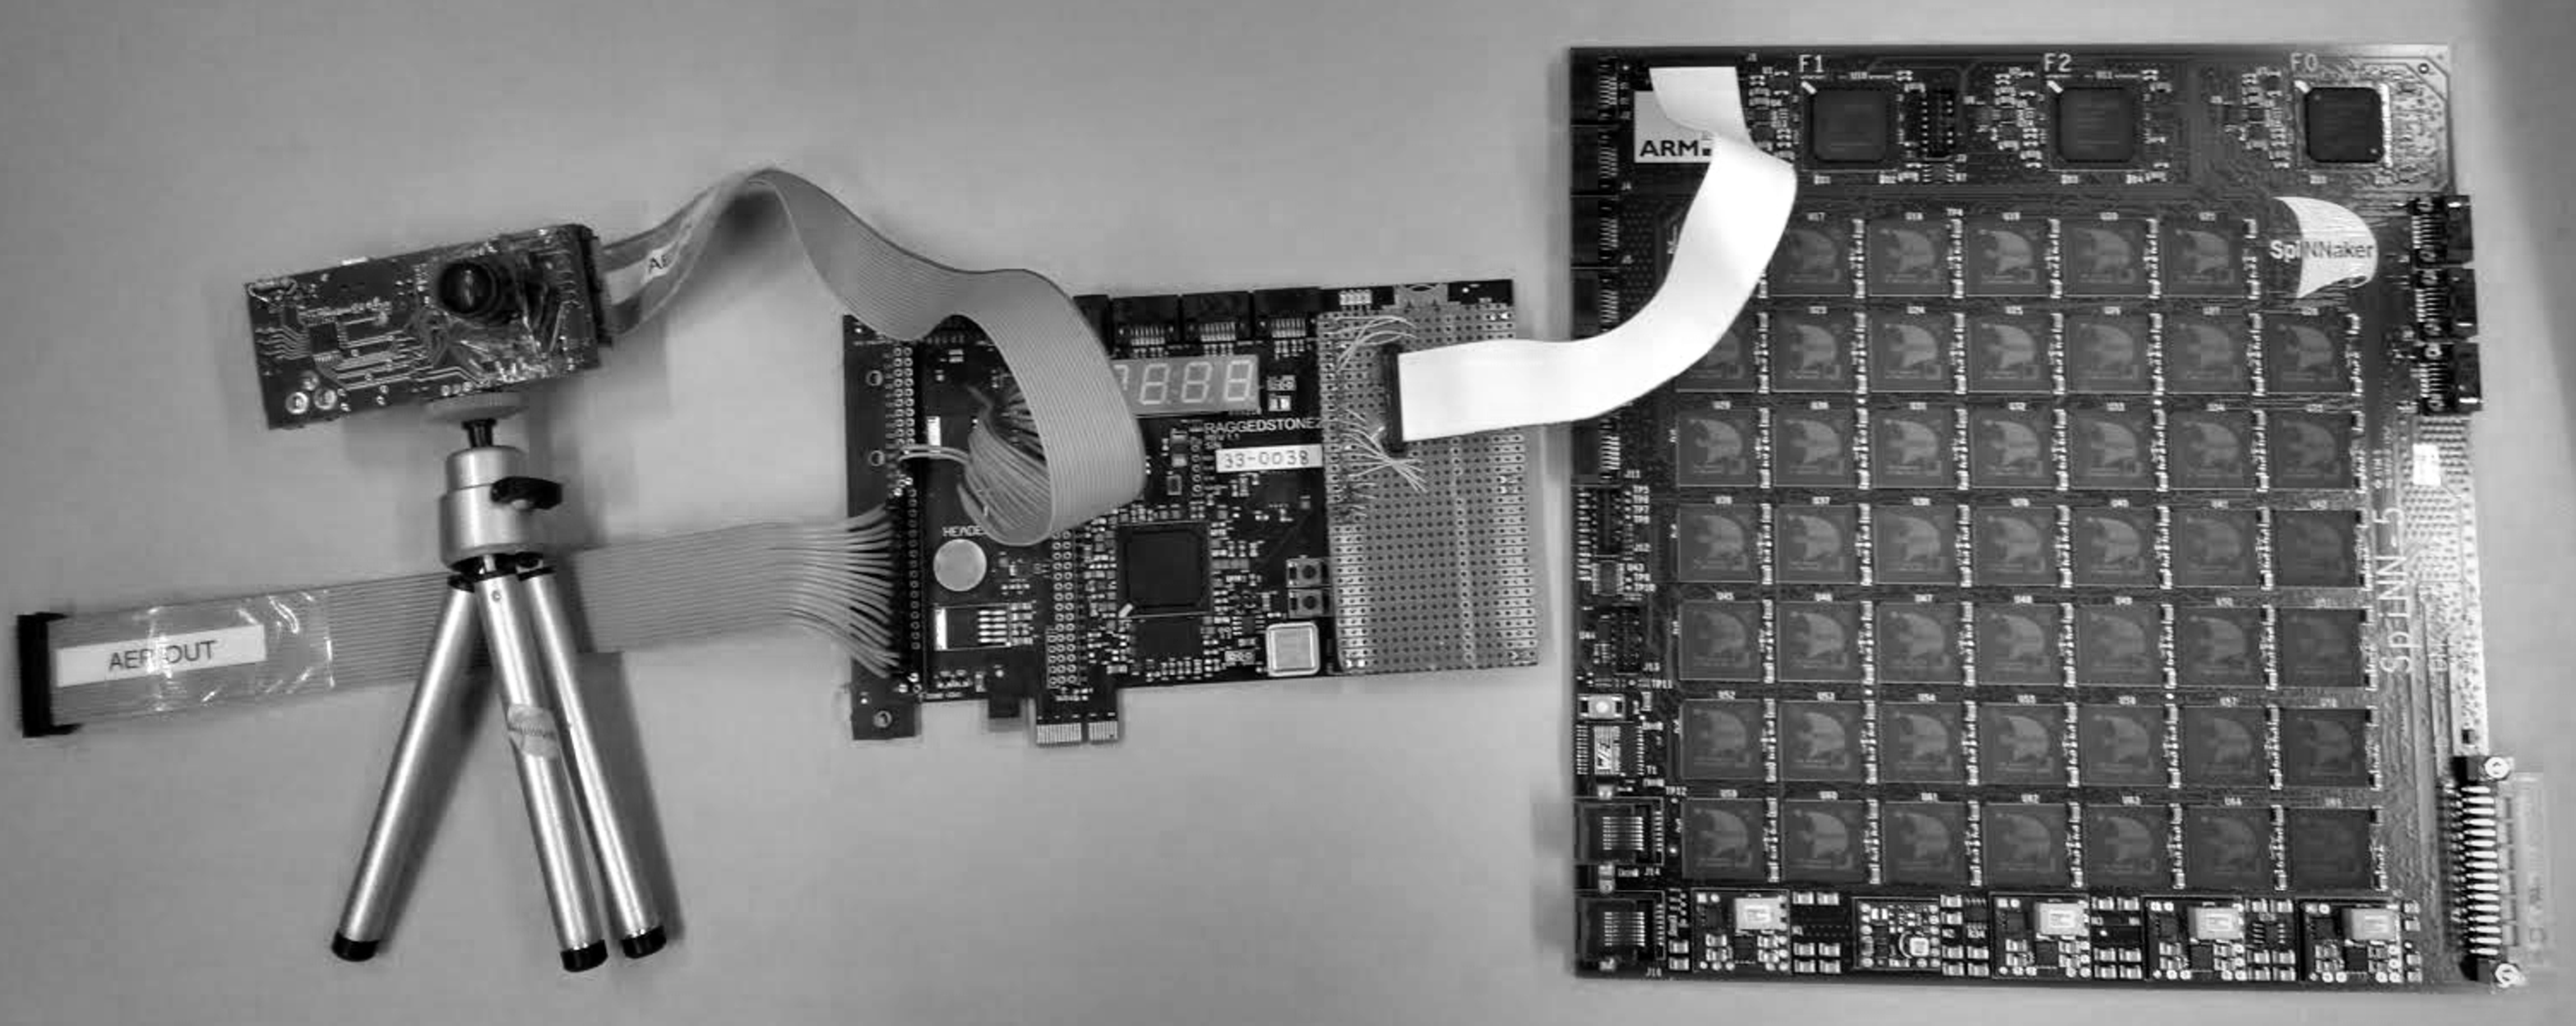
\includegraphics[width=\textwidth]{pics/outline2.pdf}	    \caption{Picture of the hardware platform. From left to right: a silicon retina, a FPGA board, and a 48-node SpiNNaker system.}
	    \label{fig:SysOverViewb}
	\end{subfigure}	

\caption{System overview of the object recognition platform. 
%The silicon retina connects to the SpiNNaker system through an FPGA board. 
%Spikes from the retina are streamed to the SpiNNaker system through this Spartan-6 FPGA board.
%The jAER software configures the retina and displays its outgoing spikes through the USB connection.
%The host sets up the runtime parameters off-line and downloads the network model to the SpiNNaker system.
}
\label{fig:SysOverView}
\end{figure}


\textbf{Vision Processing Front-ends.}
The visual input is captured by a DVS silicon retina, which is quite different from conventional video cameras.
Each pixel generates spikes when its change in brightness reaches a defined threshold.
Thus, instead of buffering video into frames, the activity of pixels is sent out and processed continuously with time.
The communication bandwidth is therefore optimised by sending activity only, which is encoded as pixel events using Address-Event Representation (AER~\cite{lazzaro1995multi}) protocol.
The level of activity depends on the contrast change; pixels generate spikes faster and more frequently when they are subject to more active change.
The sensor is capable of capturing very fast moving objects (e.g., up to 10 K rotations per second), which is equivalent to 100 K conventional frames per second~\cite{lenero20113}.

\textbf{SNNs Back-ends.}
The SpiNNaker project's architecture mimics the human brain's biological structure and functionality. 
This offers the possibility of utilizing massive parallelism and redundancy, as the brain, to provide resilience in an environment of unreliability and failure of individual components.

In the human brain, communication between its computing elements, or neurons, is achieved by the transmission of electrical `spikes' along connecting axons. 
The biological processing of the neuron can be modelled by a digital processor and the axon connectivity can be represented by messages, or information packets, transmitted between a large number of processors which emulate the parallel operation of the billions of neurons comprising the brain.

\subsection{CNN Nodels}
There are two CNNs proposed to accomplish the dynamic hand posture recognition task.
A straight forward method of template matching is employed at first, followed by a network of multi-layer perceptrons (MLP) trained to improve the recognition performance.

\begin{figure}
\centering
	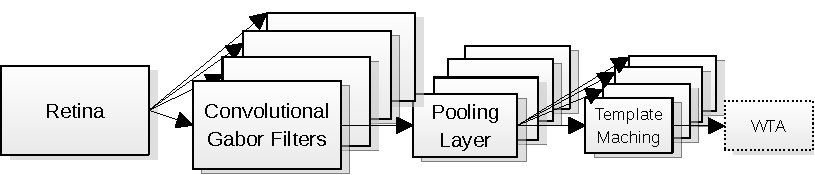
\includegraphics[width=0.48\textwidth]{pics/model1.pdf}
	\caption{Model 1. 
	The retina input is convolved with Gabor filters in the second layer, and then shrinks the sizes in the pooling layer.
	The templates are considered as convolution kernels in the last layer.
	The WTA circuit can be used as an option to show the template matching result more clearly.
	}
	\label{fig:model1}
\end{figure}
%\subsubsection{Model 1. Template Matching}

\textbf{Model 1: }
Template Matching. Shown in Figure~\ref{fig:model1} the first layer is the retina input, followed by the convolutional layer, where the kernels are Gabor filters responding to edges of four orientations.
The third layer is the pooling layer where the size of the populations shrinks. 
This down-sampling enables robust classification due to its tolerance to variations in the precise shape of the input. 
The fourth layer is another convolution layer where the output from the pooling layer is convolved with the templates.
The optional layer of Winner-Take-All (WTA) neurons enables a clearer classification result due to the inhibition between the neurons.
In the Matlab simulation, the retina input spikes are buffered into 30~ms frames, and the neurons are simple linear perceptrons.
The templates are chosen by sampling the output of the pooling layer when given some reference stimulus, see Figure~\ref{fig:template}.

\begin{figure}
\centering
	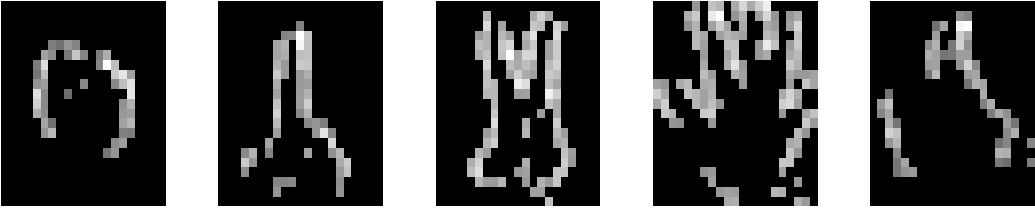
\includegraphics[width=0.48\textwidth]{pics/gesture.pdf}
	\caption{Templates of the five postures: `Fist',`Index Finger', `Victory Sign', `Full Hand' and `Thumb up'.}
	\label{fig:template}
\end{figure}

\textbf{Model 2: }
Trained MLP. 
Inspired by the research of Lecun~\cite{lecun1998gradient}, we designed a combined network model with MLP and CNN (Figure~\ref{fig:model2}). 
The first three layers are exactly the same as the previous model.
The training images for the 3-layered MLP are of same size and the posture is centred in the images.
Therefore, a tracking layer plays an important role to find the most active region and forward the centred image to the next layer.

\begin{figure}
\centering
	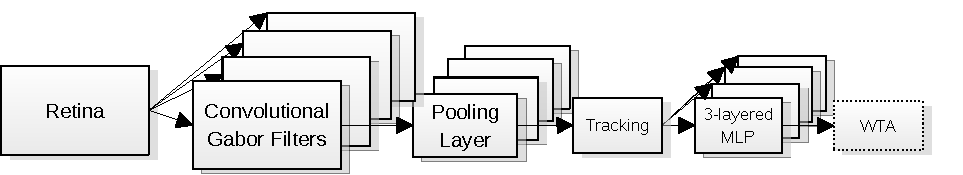
\includegraphics[width=0.5\textwidth]{pics/model2.pdf}
	\caption{Model 2. 
	The retina input convolves with Gabor filters in the second layer, and then shrinks the sizes in the pooling layer.
	The following tracking layer finds the most active area of some fixed size, moves the posture to the centre and pushes the image to the trained MLP.
	The winner-take-all (WTA) layer can be used as an option to show the template matching result more clearly.}
	\label{fig:model2}
\end{figure}

\subsection{Moving from Perceptrons to Spiking Neurons}
It remains a challenge to transform traditional artificial neural networks into spiking ones.
There are attempts~\cite{la2008response}~\cite{burkitt2006review} to estimate the output firing rate of the LIF neurons (Equation~\ref{equ:lif}) under certain conditions. 
%For the model illustrated above, there are two types of synaptic connection: one-to-one connections in the retina layer and N-to-one connections in all the convolutional layers (the pooling layer is also included). 
%For the retina layer, 1) the problem is: what is the connection weight between two single LIF neurons to make a post-synaptic neuron fire whenever the pre-synaptic neuron generates a spike? 
%While for the convolutional neurons, 2) given the input spike rates, LIF neuron parameters and the output spiking rate, what are the corresponding weights between the two layers?
\begin{equation}
\frac{\D \: V(t)}{\D\:  t}=-\frac{V(t)-V_\mathit{rest}}{\tau_m}+\frac{I(t)}{C_m}
\label{equ:lif}
\end{equation}
The membrane potential $V$ changes in response to input current $I$, starting at the resting membrane potential  $V_{rest}$, where the membrane time constant is $\tau_m = R_mC_m$, $R_m$ is the membrane resistance and $C_m$ is the membrane capacitance.

Given a constant current injection $I$, the response function, i.e. firing rate, of the LIF neuron is
\begin{equation}
\lambda_\mathit{out}=
\left [ t_\mathit{ref}-\tau_m\ln \left ( 1-\frac{V_{th}-V_\mathit{rest}}{IR_m}  \right )\right ]^{-1}
\label{equ:consI}
\end{equation}
when $IR_m>V_{th}-V_{rest}$, otherwise the membrane potential cannot reach the threshold $V_{th}$ and the output firing rate is zero. 
The absolute refractory period $t_\mathit{ref}$ is included, where all input during this period is invalid.
In a more realistic scenario, the post-synaptic potentials (PSPs) are triggered by the spikes generated from the neuron's pre-synaptic neurons other than a constant current.
Assume that the synaptic inputs are Poisson spike trains, the membrane potential of the LIF neuron is considered as a diffusion process. Equation~\ref{equ:lif} can be modelled as a stochastic differential equation referring to Ornstein-Uhlenbeck process,
\begin{equation}
\tau_m\frac{\D\:V(t)}{\D\:  t}=-\left[V(t)-V_\mathit{rest}\right] + \mu + \sigma\sqrt{2\tau_m}\xi (t)
\label{equ:sde}
\end{equation}
where
\begin{equation}
\begin{array}{l}
\mu=\tau_m(\mathbf{w_E\cdot\lambda_E}-\mathbf{w_I\cdot\lambda_I})
\\
\\
\sigma ^{2} = \frac{\tau_m}{2}\left(\mathbf{w_E^{2}\cdot\lambda_E}+\mathbf{w_I^{2}\cdot\lambda_I}\right)
\end{array}
\label{equ:ou}
\end{equation}
are the conditional mean and variance of the membrane potential.
The delta-correlated process $\xi(t)$ is Gaussian white noise with zero mean, $\mathbf{w_E}$ and $\mathbf{w_I}$ stand for the weight vectors of the excitatory and the inhibitory synapses, and $\mathbf{\lambda}$ represents the vector of the input firing rate.
The response function of the LIF neuron with Poisson input spike trains is given by the Siegert function~\cite{siegert1951first}, 
\begin{align}
\lambda_\mathit{out} &=\left(\tau_\mathit{ref} + \frac{\tau_Q}{\sigma_Q}\sqrt{\frac{\pi}{2}} \int_{V_\mathit{rest}}^{V_\mathit{th}}\D\,u \:\exp \left(\frac{u-\mu_Q}{\sqrt2\sigma_Q} \right )^{2} \right. \nonumber \\
&\qquad \left. \vphantom{\int_t} \cdot  \left[1+\mathrm{erf} \left(\frac{u-\mu_Q}{\sqrt2\sigma_Q} \right ) \right ]\right)^{-1}
\label{equ:sgt}
\end{align}
%\begin{align}
%\lambda_\mathit{out} &=\left(\tau_\mathit{ref} + \frac{\tau_Q}{\sigma_Q}\sqrt{\frac{\pi}{2}} \int_{V_\mathit{rest}}^{V_\mathit{th}}\D\,u \:\exp \left(\frac{u-\mu_Q}{\sqrt2\sigma_Q} \right )^{2} \right. \nonumber \\
%&\qquad \left. \vphantom{\int_t} \cdot  \left[1+\mathrm{erf} \left(\frac{u-\mu_Q}{\sqrt2\sigma_Q} \right ) \right ]\right)^{-1}
%\label{equ:sgt}
%\end{align}
where $\tau_Q, \mu_Q, \sigma_Q$ are identical to $\tau_m, \mu, \sigma$ in Equation~\ref{equ:ou}, and erf is the error function.

Still there are some limitations on the response function. 
For the diffusion process, only small amplitude (weight) of the PostSynaptic Potentials (PSPs) generated by a large amount of input spikes (high spiking rate) work under this circumstance; 
plus, the delta function is required, i.e. the synaptic time constant is considered to be zero. Thus only a rough approximation of the output spike rate has been determined.
Secondly, given different input spike rate to each pre-synaptic neurons, the parameters of the LIF neuron and the output spiking rate, how to tune every single corresponding synaptic weight remains a difficult task.

\subsection{Experiments}
\textbf{Experiment Set-up.}
In order to evaluate the cost and performance trade-offs in optimizing the number of neural components, both the convolutional models described above are tested at different scales. 
Five videos of every posture are captured from the silicon retina in AER format, all of similar size and moving clock-wise in front of the retina. 
The videos are cut into frames (30~ms per frame) and presented to the convolutional networks. 

Model 1 is tested on both percetrons in Matlab and LIF neurons on SpiNNaker;
whereas, Model 2 is only validated on Matlab since it merely estimates the highest performance of the system but in a non-biological way.
All the details can be found in the latest submitted paper.

\textbf{Recognition using LIF neurons.}
The output spikes generated from the recognition populations with time are shown in Figures~\ref{fig:rps} for full resolution system. 
More spikes are generated during the period when the preferred input posture is shown. 


\begin{figure}[h!]
\centering
	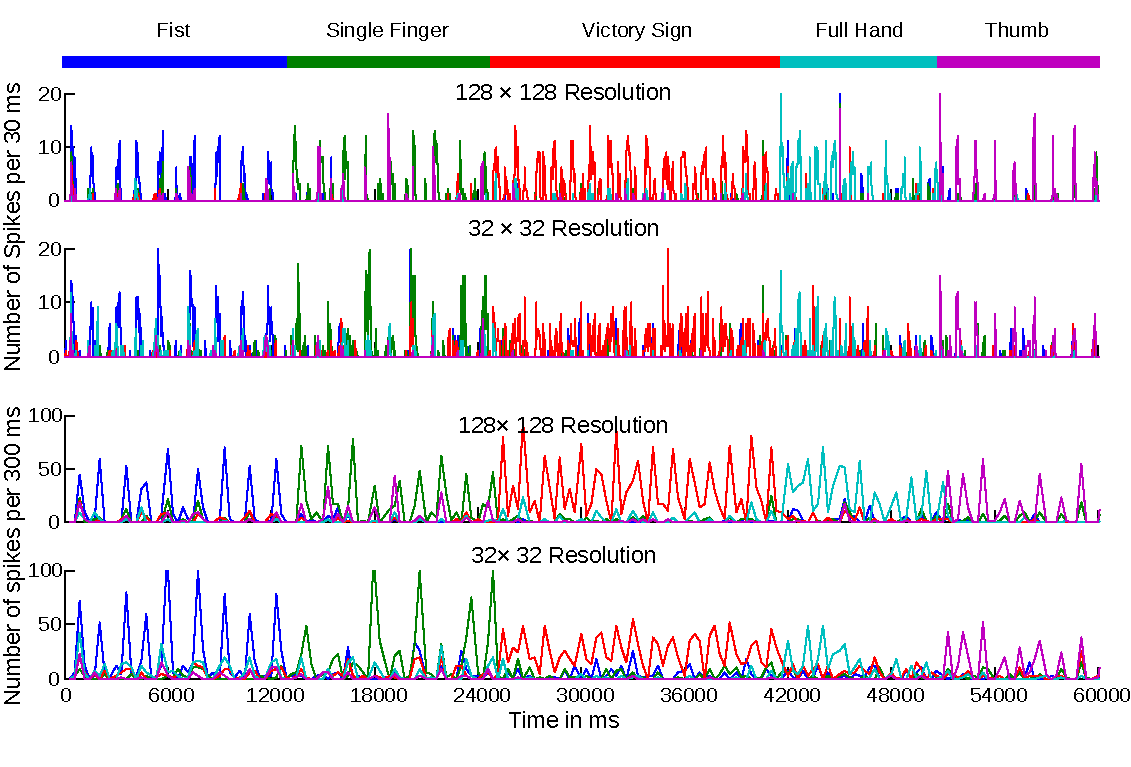
\includegraphics[width=0.48\textwidth]{pics/rateSpiNN.pdf}
	\caption{Real-time neural responses of two experiments on SpiNNaker with time to recorded postures.
	These two experiments only differ in input resolution.
%	The result of the high input resolution test is plotted the first with a sample frame of 30~ms; 
%	while the 3rd plot shows the same result with a sample frame of 300~ms.
%	The other two plots refer to the smaller input resolution.
	Every point represents the over all number of spikes of a specific population (different colour) in a `frame'.
	First two plots are for a sample frame of 30~ms; the latter are for a frame of 300~ms.
	}
	\label{fig:spikerec}
\end{figure}

\begin{figure}
\centering
	\begin{subfigure}[t]{0.24\textwidth}
		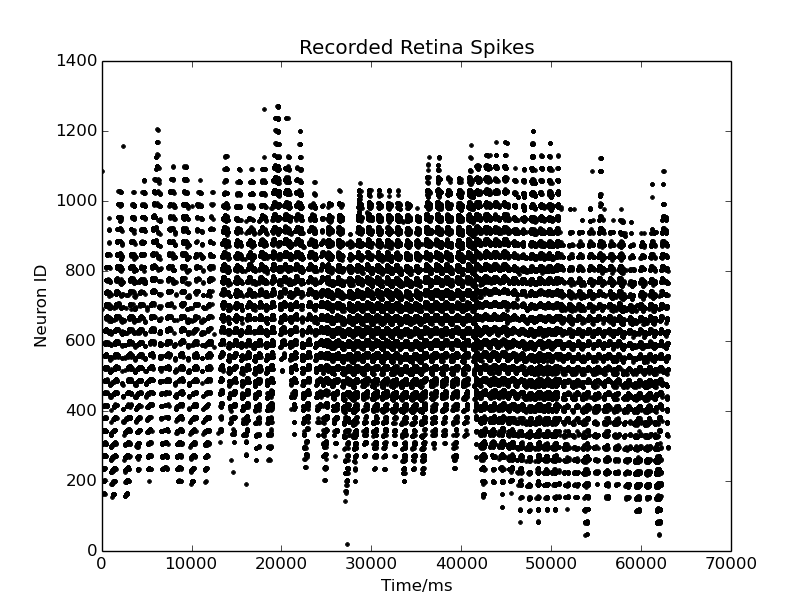
\includegraphics[width=\textwidth]{pics/figure_r.png}
	    \caption{Retinal input population }
	    \label{fig:ssa}
	\end{subfigure}
	\begin{subfigure}[t]{0.24\textwidth}
		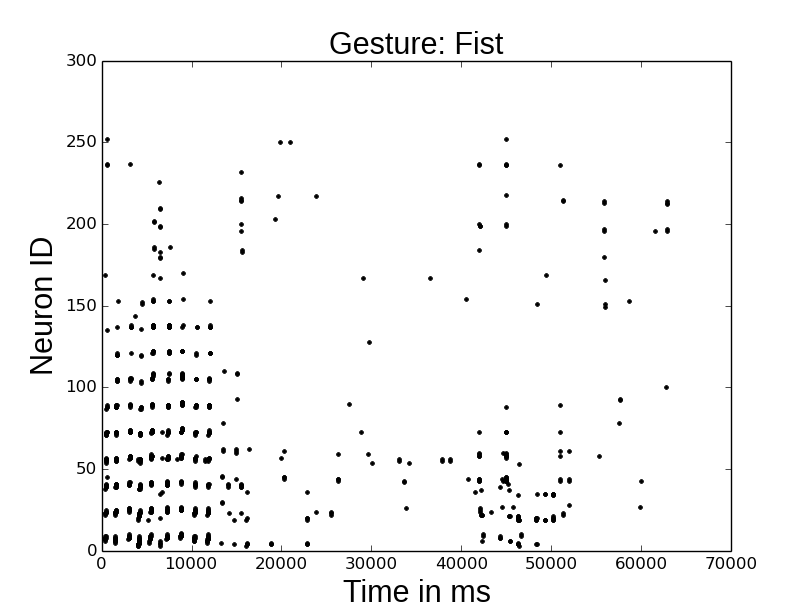
\includegraphics[width=\textwidth]{pics/figure_1.png}
		\caption{Template matching population, `Fist'}
	    \label{fig:rec0}
	\end{subfigure}
	\\
	\begin{subfigure}[t]{0.24\textwidth}
		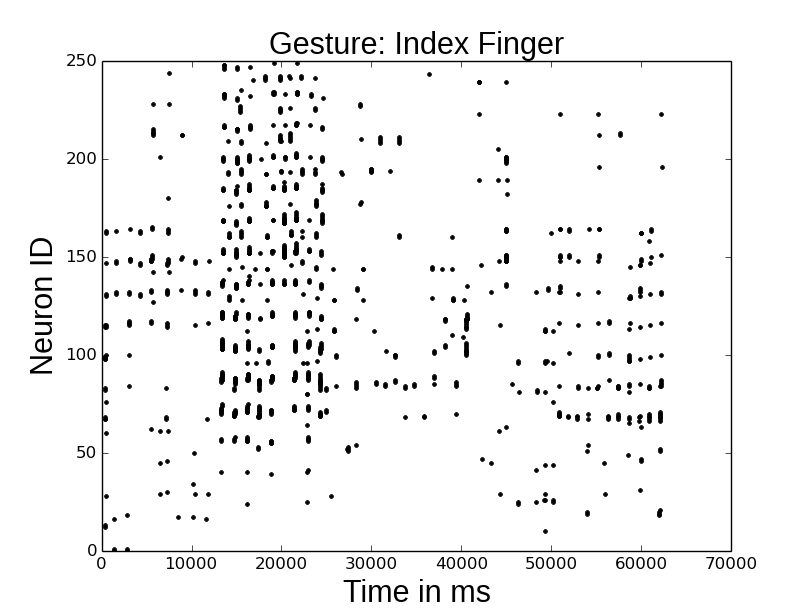
\includegraphics[width=\textwidth]{pics/figure_2.png}
		\caption{Template matching population, `Index Finger'}
	    \label{fig:rec1}
	\end{subfigure}	
	\begin{subfigure}[t]{0.24\textwidth}
		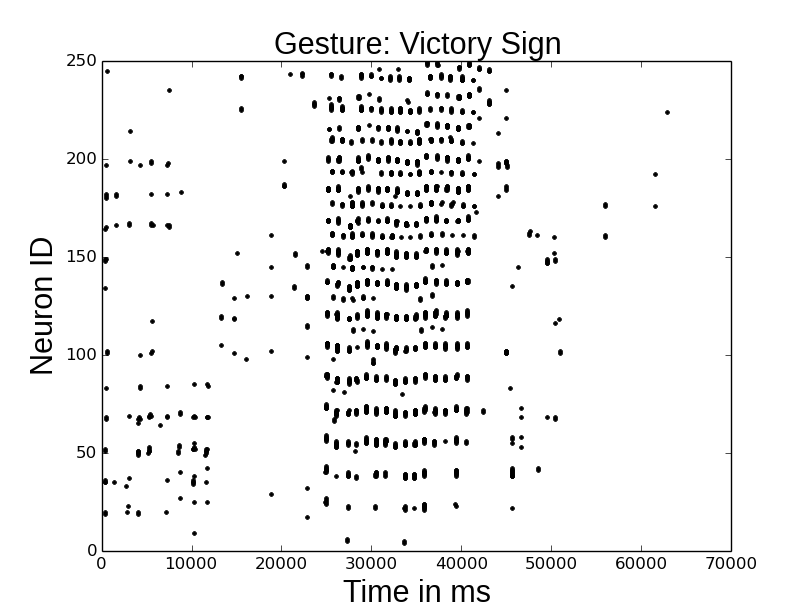
\includegraphics[width=\textwidth]{pics/figure_3.png}
		\caption{Template matching population, `Victory Sign'}
	\end{subfigure}	
	\\
	\begin{subfigure}[t]{0.24\textwidth}
		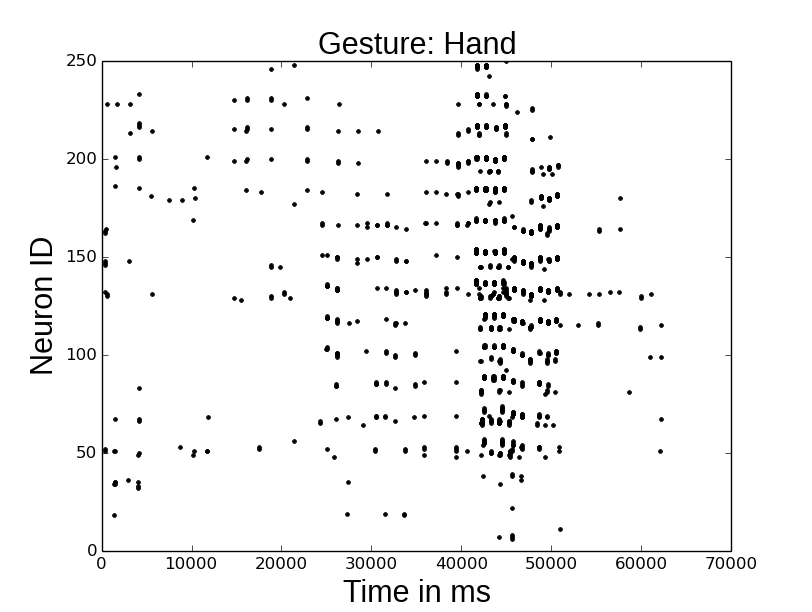
\includegraphics[width=\textwidth]{pics/figure_4.png}
		\caption{Template matching population, `Full Hand'}
	    \label{fig:rec5}
	\end{subfigure}	
	\begin{subfigure}[t]{0.24\textwidth}
		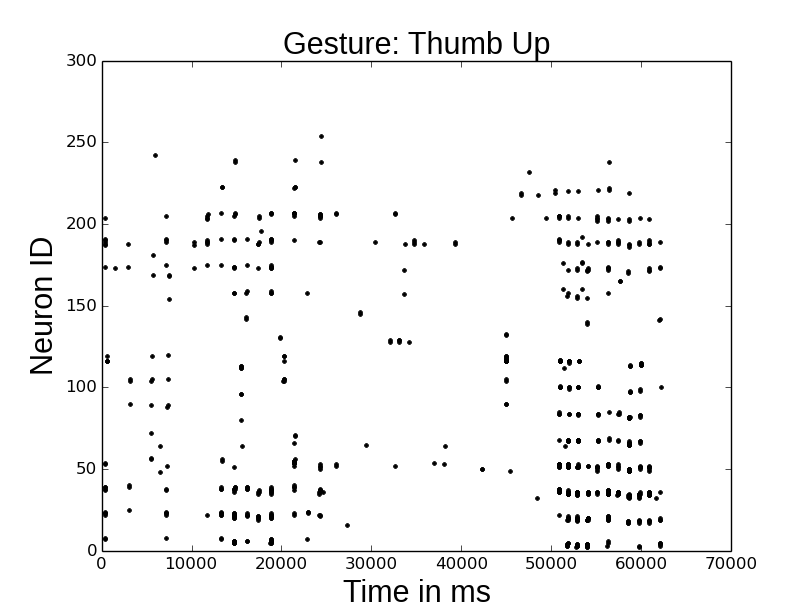
\includegraphics[width=\textwidth]{pics/figure_5.png}
		\caption{Template matching population, `Thumb Up'}
	    \label{fig:rect}
	\end{subfigure}	
\caption{Spikes captured during the live recognition of the recorded retinal input with the resolution of 128$\times$128. }
\label{fig:rps}
\end{figure}
%\begin{figure}
%\centering
%	\begin{subfigure}[t]{0.24\textwidth}
%		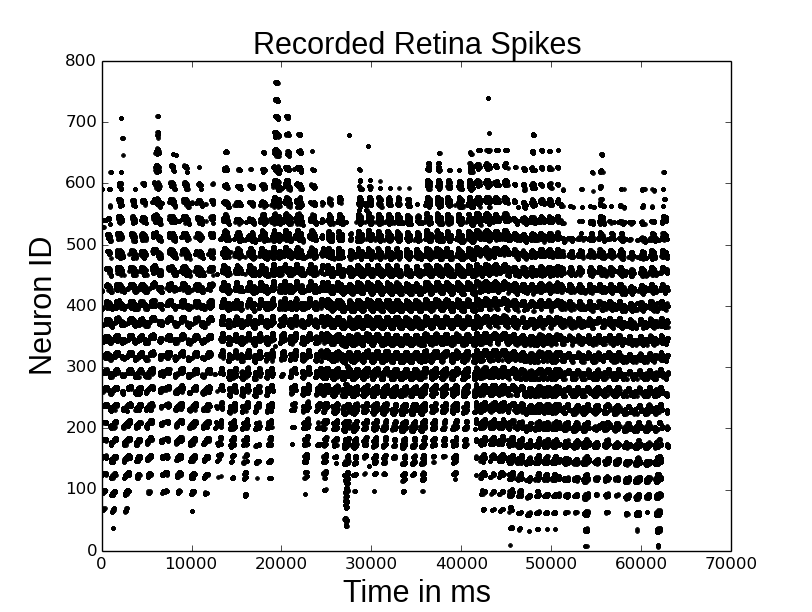
\includegraphics[width=\textwidth]{pics/figure_32_r.png}
%	    \caption{Retinal input population }
%	    \label{fig:ssa32}
%	\end{subfigure}
%	\begin{subfigure}[t]{0.24\textwidth}
%		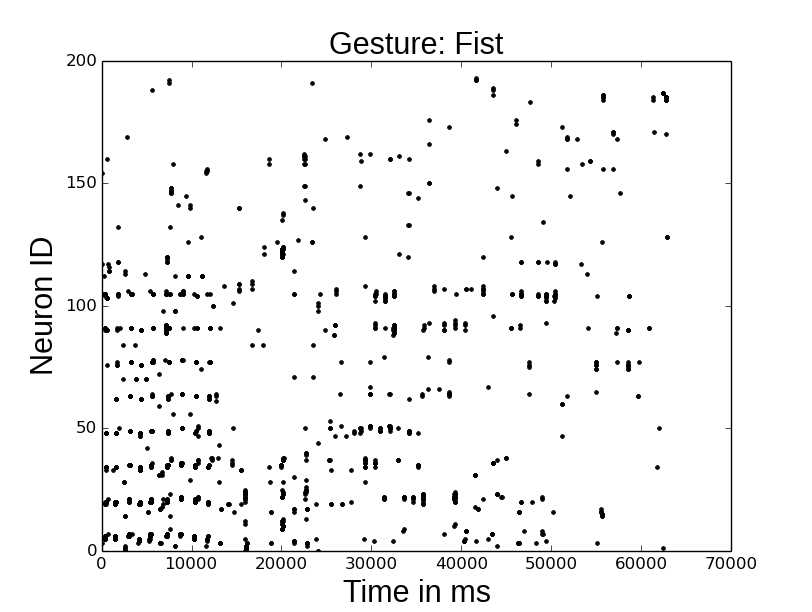
\includegraphics[width=\textwidth]{pics/figure_32_1.png}
%		\caption{Template matching population, `Fist'}
%	    \label{fig:rec032}
%	\end{subfigure}
%	\\
%	\begin{subfigure}[t]{0.24\textwidth}
%		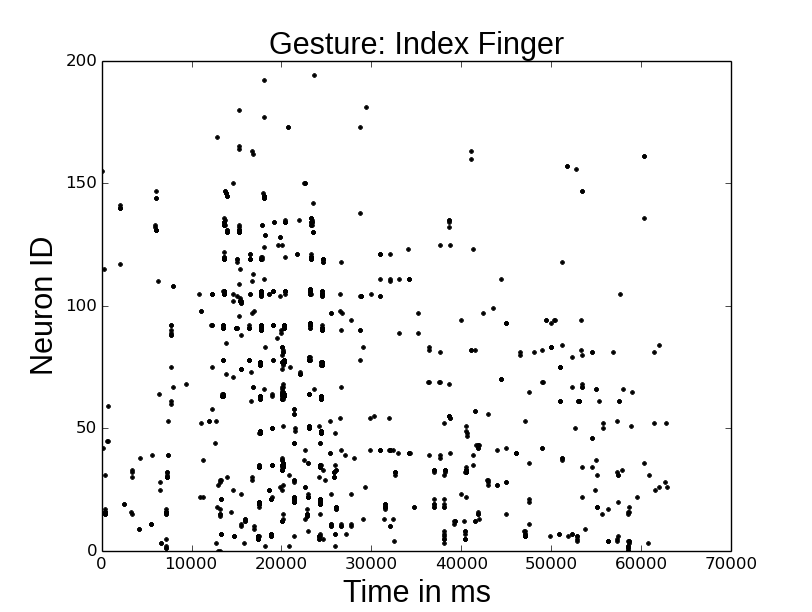
\includegraphics[width=\textwidth]{pics/figure_32_2.png}
%		\caption{Template matching population, `Index Finger'}
%	    \label{fig:rec132}
%	\end{subfigure}	
%	\begin{subfigure}[t]{0.24\textwidth}
%		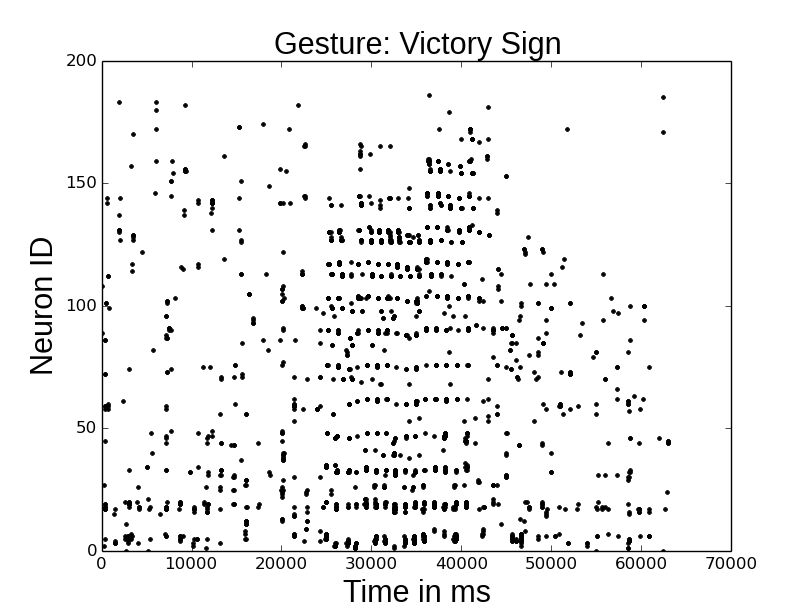
\includegraphics[width=\textwidth]{pics/figure_32_3.png}
%		\caption{Template matching population, `Victory Sign'}
%	\end{subfigure}	
%	\\
%	\begin{subfigure}[t]{0.24\textwidth}
%		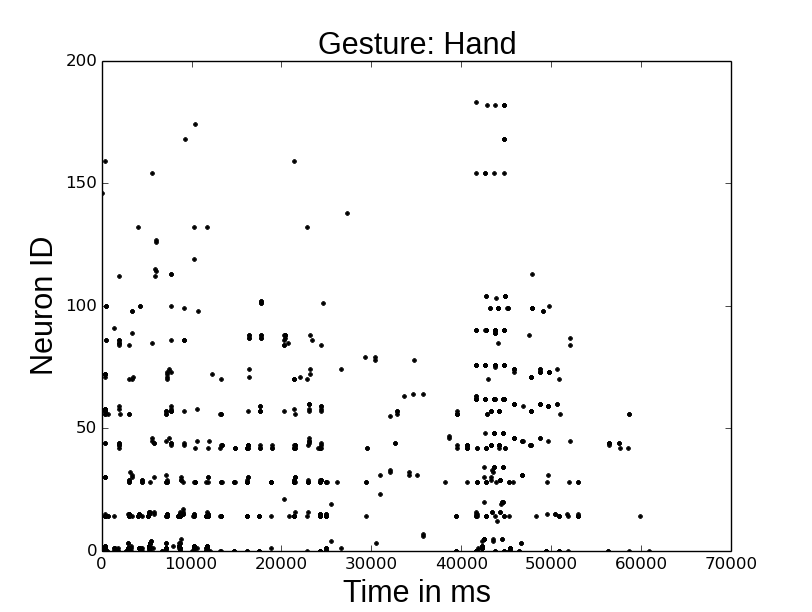
\includegraphics[width=\textwidth]{pics/figure_32_4.png}
%		\caption{Template matching population, `Full Hand'}
%	    \label{fig:rec532}
%	\end{subfigure}	
%	\begin{subfigure}[t]{0.24\textwidth}
%		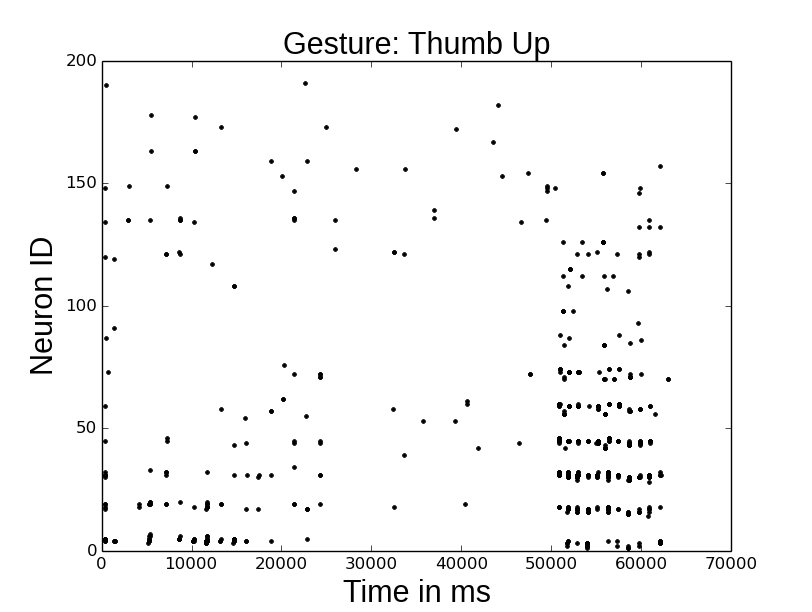
\includegraphics[width=\textwidth]{pics/figure_32_5.png}
%		\caption{Template matching population, `Thumb Up'}
%	    \label{fig:rect32}
%	\end{subfigure}	
%\caption{Spikes captured during the live recognition of the recorded retinal input with the resolution of 32$\times$32. }
%\label{fig:rps32}
%\end{figure}

In this study's largest configuration using these approaches, a network of 74,210 neurons and 15,216,512 synapses is created and operated in real-time using 290 SpiNNaker processor cores in parallel and with 93.0\% accuracy.
A smaller network using only 1/10th of the resources is also created, again operating in real-time, and it is able to recognise the postures with an accuracy of around 86.4\% - only 6.6\% lower than the much larger system.
The recognition rate of the smaller network developed on this neuromorphic system is sufficient for a successful hand posture recognition system, and demonstrates a much improved cost to performance trade-off in its approach.

\section{Future Work} 
\begin{figure}[h!]
	\centering
	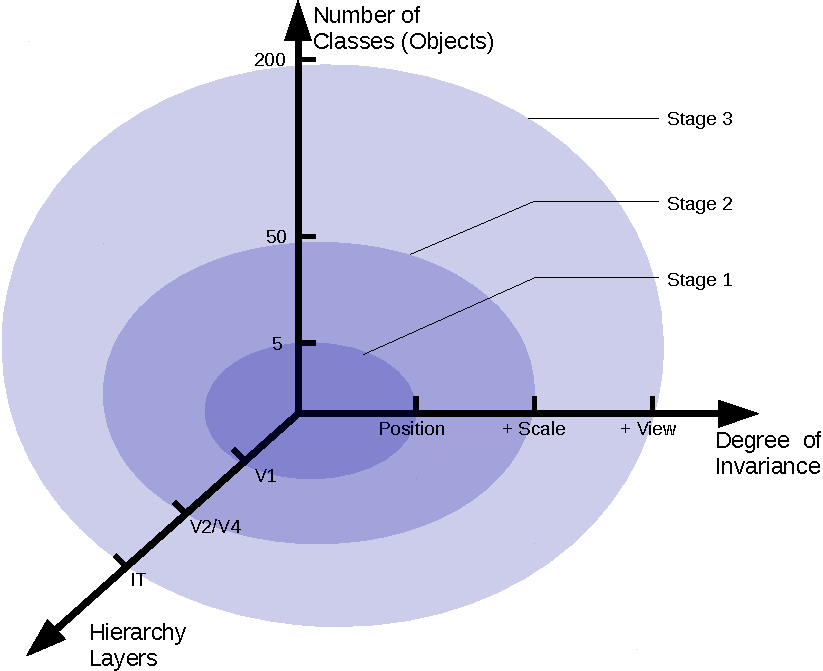
\includegraphics[width=0.48\textwidth]{pics/stages.pdf}
	\caption{3D representation of the research plan on the transformation-invariant object recognition system.
	Three milestones are pointed out indicating the expected targets of the object recognition networks.
	}
	\label{Fig:3Dplan}
\end{figure}
The proposed research plan is illustrated in Figure~\ref{Fig:3Dplan}, where the scope of the research is estimated in three dimensions.
To build a biologically-plausible object recognition system using spiking neurons, this work will be completed in three stages:
\begin{enumerate}
	\item Year 1, building a position-invariant object recognition system exploiting V1-like neurons to classify five hand postures. 
	\item Year 1.5, combining scale- with position-invariance on the object recognition system, and building the hierarchy ventral pathway to the V2/V4 layer to recognise 50 simple combined features such as gratings and contours.
	\item Year 2.5. integrating position-, scale- and view-invariance by modelling the hierarchical visual pathway up to the IT cortex and equipping the system with the ability to recognise 200 objects in real time.
\end{enumerate}
%The recognition ability of the system is measured in three dimensions: the hierarchy layers, degree of invariance and the network size.
 
This work will contribute to the understanding of biological visual processing by means of mimicking the neural activities in the ventral stream.
More importantly, the research will apply the accurate, rapid and robust approaches to artificial systems by exploring the brain's invariant object recognition.
The performance of the real-time recognition system will be tested on each milestone to validate the success of the models.
The neural activities and recognition rate will also be compared with biological data.

The key research steps are listed in Figure~\ref{Fig:gantt}.
Since the incremental work flow is hard to present in Gantt charts, only the work for the first milestone is shown.
The subsequent sections will outline the key research stages.



\begin{figure}[h!]
	\centering
	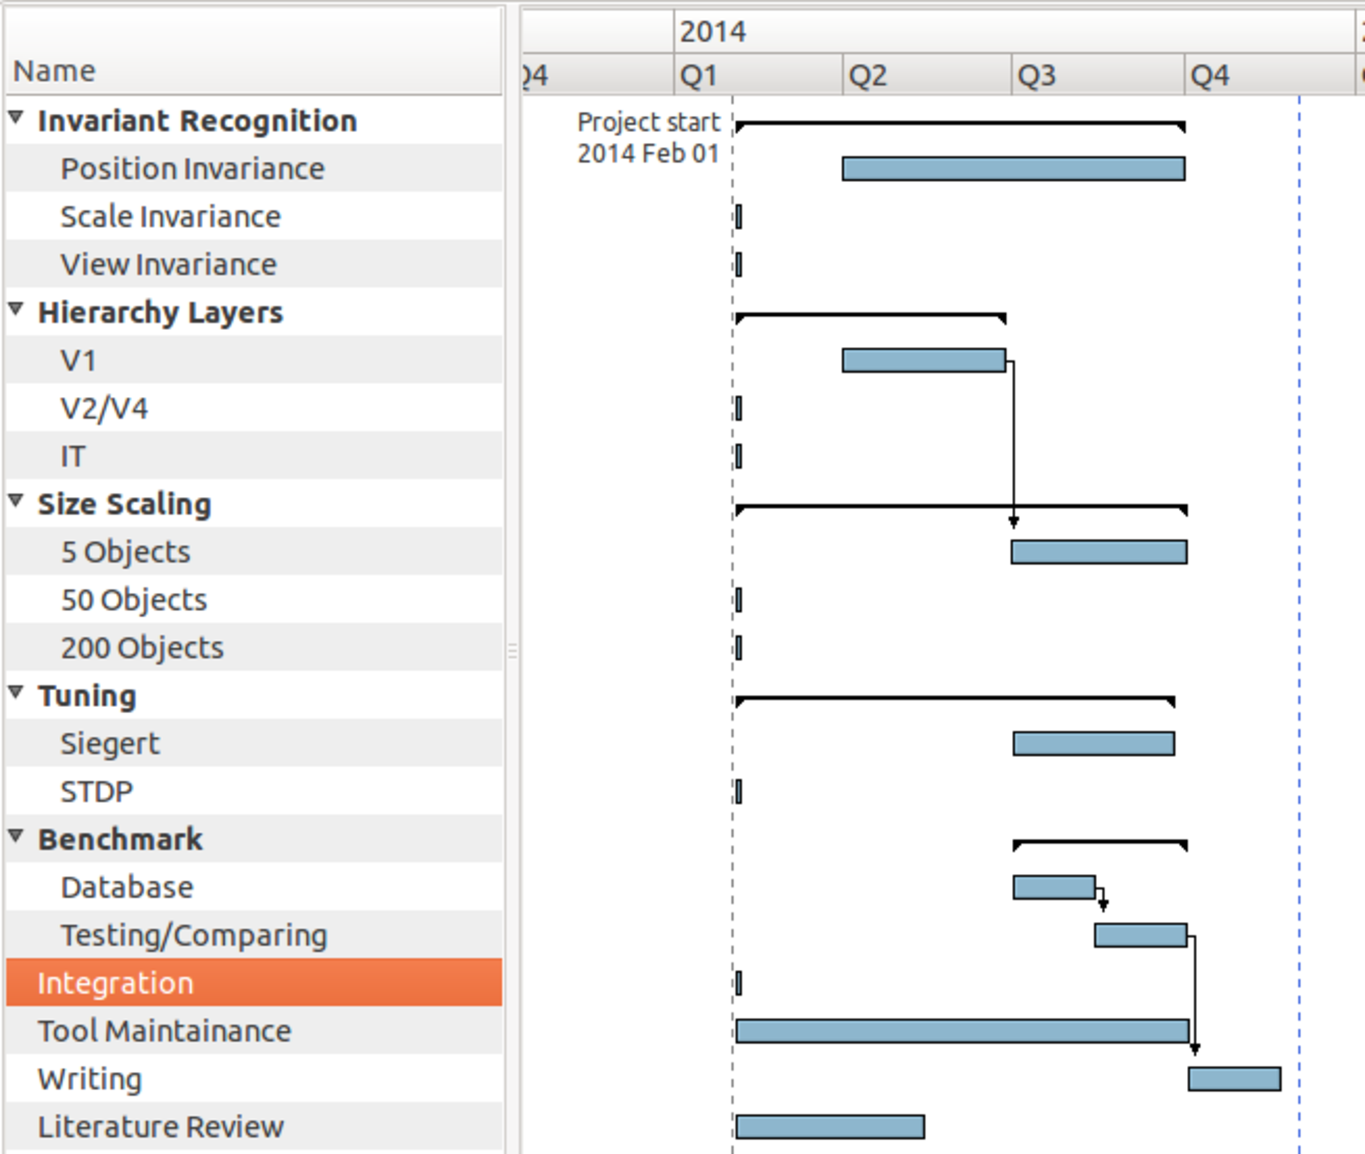
\includegraphics[width=0.48\textwidth]{pics/gantt.pdf}
	\caption{Gantt chart of the work flow for the first milestone.
	The main research works are listed on the left.
%	Different from the example, in the following work, not only achieving a milestone but also any increase in any dimension will result in tuning and benchmark testing.
	}
	\label{Fig:gantt}
\end{figure}
\subsection{Invariant Object Recognition}
As stated previously the brain recognises huge number of objects rapidly with ease even in noisy natural scenes. We will explore the invariant object recognition in three features: position, scale and viewing angle.
%While the major stumbling crux of the computer object recognition systems lies in the invariance problem.
%To explore the invariant object recognition of the brain in a biologically plausible way is the right place to solve the computational difficulty.
\subsubsection{Position Invariance}
Position invariance in the lower level of V1-liked neurons has been achieved in the preliminary work by convolving receptive fields with Gabor kernels.
The following work in accordance with Figure~\ref{Fig:3Dplan} will focus on expanding the position invariance to higher hierarchical levels of the ventral stream.
\subsubsection{Scale Invariance}
Similar to orientation detection, V1 provides overcomplete population re-representations of visual image on the features of scale, frequency and orientation.
It forms the basis of scale invariant object recognitions.
Likewise, integrating the features into the higher abstraction of layered network to recognise more complex figures will require a tense work on tuning.
\subsubsection{View Invariance}
A difficult specificity-invariance trade-off occurs in view invariant recognition tasks, since the recogniser should be able to discriminate different objects while at the same time also tolerating to viewing angle transformations.
Learning will play a very important role in this work, where objects observed with multiple view points can be recognised even if only single view point is presented during training.
\subsection{Modelling the Ventral Visual Pathway}
As the visual information propagates through the ventral stream (via visual area V1, V2/V4 and IT), neurons become selective for increasingly complex features. 
Along with this growing complexity of the preferred stimulus, neurons become more and more tolerant to the position and scale of the stimulus within their receptive fields.
Inspired from the functional behaviour of the biological data (many have been mentioned in Section~\ref{sec:bio}), this work will mimic the neural activity of each hierarchy layer by LIF neurons.
 
%To satisfy the functional discoveries, this work will employ learning and compare with biological data.
%This work will ask for a close collaboration with neuroscience to gather biological data for both training and testing.
\subsection{Size Scaling}
The milestones set for the dimension of number of classes/objects is in accordance with experimental data from the study of neuroscience.
In work by~\cite{hegde2004temporal}, the classical receptive field of the V2 cell consists of 48 grating stimuli and 80 contour stimuli; while Zoccolan et al.~\cite{zoccolan2007trade} tested and recorded the activity of the IT neurons of monkeys with 213 grayscale pictures of isolated real-world objects.

Thanks to the massively-parallel neural simulations possible in the SpiNNaker system, implementing real-time invariant object recognition becomes possible.
However, it also requires the supporting software development to support larger neural networks than currently possible.  
\subsection{Integration}
To reach the milestone of building an object recognition system with position, scale and view invariance, integration of these separate models will be a challenge.
It not only requires placing the models physically together but also merging their functions.
As illustrated in Section~\ref{sec:bio}, single neurons are tuned to different features and object identities.
This work requires further investigation into population coding and learning. 
\subsection{Tuning}
Tuning is the key to make the object recognition system a success.
In preliminary work, Siegert transformation functions are used to adjust perceptral weights for spiking LIF neurons.
This is a strong indicator of the feasibility of the work.
However, learning algorithms such as STDP in spiking neural networks are must be employed to make the system more biologically plausible.
It is hoped that, this work will provoke further study of learning algorithms on SpiNNaker.
\subsection{Benchmarking Performance}
The performance of the real-time recognition system will be evaluated of each milestone to validate the success of the models.
The neural activities and recognition rate will be compared with biological data which will act as a benchmark.
\subsubsection{Building a Dataset}
Building a well-labelled retinal output dataset is essential in spike-based object recognition study.
Unified benchmarks with AER format will be ideal for SNN study, because of its non-frame, event-based fashion.
These benchmark datasets will also make it possible for other researchers to test their SNN model without a silicon retina present.
%It is hoped that this would boost communication, comparison and collaboration within the community.
%This work also requires lively discussion and cooperation with neuroscientists, where data can be derived and tested.
\subsubsection{Testing/Comparing}
The testing and comparing on the dataset will verify the reliability of the models.
The neural responses of single or populated neurons to the same dataset will be analysed in firing rate and response time.
By comparing with the biological data, the model can be rectified and improved.
The more data it compares with, the closer it could untangle the object representation. 

\bibliography{refs}    % this causes the references to be listed
\bibliographystyle{ieeetr}

%\end{biography}
\end{document}
